% Summary of deal2025: Current models of {Agree}

\begin{abstract}
Merge and Agree are the only operations in syntax, Agree is triggered by Merge, and Agree isn’t built on interpretability and valuedness, but instead on interaction and satisfaction.

Insights:

\begin{itemize}
  \item Three developments have rendered the original interpretability and valuedness motivation theoretically redundant: relativized probing, default agreement, and alternatives to the Activity Condition.
  \item The strong Merge-Agree Hypothesis is that Merge and Agree are the only operations, and all non-local processes (phi-agreement, NPI licensing, etc.) are Agree.
  \item Has a good listing of the original Probe-Goal theory.
  \item Interaction/Satisfaction, but not interpretability and valuedness, is one of Preminger 2014’s Obligatory Operations.
\end{itemize}

Key empirical facts to explain:

\begin{itemize}
  \item Superiority Effects are essentially relativized minimality but tiered.
  \begin{itemize}
    \item Béjar 2003’s Chirag Dargwa cases: verbs agree only with things with [Part], but copy the specific [Spkr] or [Addr] feature.
  \end{itemize}
  \item Default Agreement
  \begin{itemize}
    \item In Chirag Dargwa, when both arguments are third person, there’s no person affix.
    \item In Hindi-Urdu, when neither argument is nominative/unmarked, agreement takes a default (identical to 3ms) form.
  \end{itemize}
  \item Hyperraising and its absence (A-movement on top of A-movement)
  \begin{itemize}
    \item In Brazilian Portuguese and Zulu, you can say things like “The boys seem that did the homework”.
    \item In English, you can’t get these - Nevins 2004 argues the BP nouns are able to escape the lower phase because they move a little bit higher than English nouns; Halpert 2016, 2019 argues that English embedded finite C bears phi-features, blocking hyperraising by relativized minimality.
  \end{itemize}
  \item Multiple Agreement
  \begin{itemize}
    \item In Hindi-Urdu, a single DP can agree with both auxiliaries and the main verb, and an embedded object DP can agree with a matrix verb like “want” in “I want to buy flowers”.
    \item Also in Tsez, Innu-Aimun, Daga, Nez Perce, and Ojibwe
    \item And in numerous Bantu languages including Kiswahili, Kilega, and Luusamia
  \end{itemize}
  \item Negative Concord, Parasitic Participles, and Sequence of Tense
  \begin{itemize}
    \item These things all seem semantically Upwards.
    \item But they could also be Downwards, if you forget about interpretability and semantics.
  \end{itemize}
\end{itemize}
\end{abstract}

\section*{Introduction}

The Merge-Agree Hypothesis (Deal's term):

\begin{itemize}
  \item There are exactly two basic operations of natural language syntax, one that holds extremely locally, under sisterhood (Merge), versus one that can operate at a distance (Agree).
\end{itemize}

If correct, all dependencies at a distance can be treated with the same operation.

Nearly all current models of such an operation have their origin in Chomsky 2000, 2001, but the term is not reserved for that algorithm.

Deal thinks Interaction/Satisfaction Theory, introduced in Deal 2015, Deal 2024, and further developed in a range of cross-linguistic work listed, is better.

The unificatory project has had great successes, but has been unmoored from its original motivation: the LF deletion of uninterpretable features.

Three stands of literature that have chipped away at this foundation, while improving the theory's empirical adequacy:

\begin{enumerate}
  \item Valuation and relativized probing
  \item Defaults and failures to value
  \item Whether goals must be made ``active'' by uninterpretable features
\end{enumerate}

Then review debate about the directionality of Agree.

Then present interaction/satisfaction theory.

\section*{Traditional Probe-Goal Agreement}

\subsection*{History}

Chomsky 2000, Chomsky 2001:3 introduces Agree motivated by a need to remove elements from a derivation that are incompatible with semantic interpretation:

\begin{quote}
The empirical facts make it clear that there are (LF-)uninterpretable inflectional features that enter into agreement relations with interpretable inflectional features. . . . The obvious conclusion, which we adopt, is that the agreement relation removes the uninterpretable features from the narrow syntax, allowing derivations to converge at LF while remaining intact for the phonological component

\end{quote}

Here Agree arises from the tension between two properties of language:

\begin{enumerate}
  \item LF needs full interpretation
  \item Some features of LIs are not semantically interpretable
\end{enumerate}

Another proposal concerning the features driving Agree connects their uninterpretability to unvaluedness (2001:5)

\begin{quote}
Uninterpretable features... enter the derivation without values, and are distinguished from interpretable features by [this].

\end{quote}

\subsection*{How it works}

Agree holds between a Probe and a Goal iff:

\begin{enumerate}
  \item \textbf{Probe specification}: the probe bears uF (uninterpretable, unvalued)
  \item \textbf{Structural condition}: the probe c-commands the goal
  \item \textbf{Match condition}: the uF of the probe matches the iF of the goal
  \item \textbf{Activity condition}: the goal is active (also has uninterpretable features)
  \item \textbf{Minimality condition}: the goal is the closest element to the probe meeting the condition above
\end{enumerate}

When Agree happens:

\begin{enumerate}
  \item \textbf{Valuation}: F's value is copied to the probe from the goal
  \item \textbf{Goal flagging}: The goal's uninterpretable features are given values according to the nature of the probe somehow
  \item \textbf{Movement}: Optionally, movement of the goal (re-merge) is triggered, depending on whether the probe has EPP or not
  \item \textbf{Deletion}: Uninterpretable features are deleted
\end{enumerate}

\section*{Superiority Effects (Valuation and Relativized Probing)}

I think Deal is just using this term to mean ``relativized minimality but tiered''.

Examples:

\begin{enumerate}
  \item English wh-objects can raise but not across wh-subjects
  \begin{itemize}
    \item probe has [uWh]
  \end{itemize}
  \item Chirag Dargwa verbs agree with the subject if it's 1st or 2nd person, but with the object when the subject is 3rd person
  \begin{itemize}
    \item probe has [uPartic]
  \end{itemize}
\end{enumerate}

One wrinkle with (2):

\begin{itemize}
  \item if the probe just had [uPartic], then presumably 1st and 2nd person agreement would be the same morphologically due to Valuation
\end{itemize}

Béjar 2003's solution:

\begin{itemize}
  \item The probes \textit{matches} based on [uPartic], but \textit{values} based on [Partic] and [Speaker].
  \item The probe copies back any sub-features of the matched feature, enumerated by feature geometry:
\end{itemize}
\begin{center}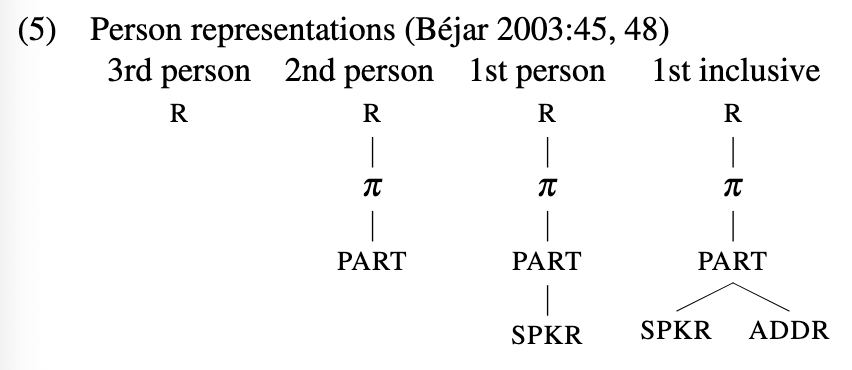
\includegraphics[width=0.50\linewidth]{images/pasted-20260921091030.png}\end{center}

Weird motivationally: if deleting [uPartic] is the motivation, then copying additional features should be superfluous.

\begin{itemize}
  \item Valuation seems increasingly separate.
\end{itemize}

Central is not even Valuation, but \textit{copying}.

Also, crucially, this only works with privative features, because then the probe would find [-Partic] on the 3rd person subject and that would delete its uninterpretable [uPartic] feature.

\section*{Defaults and Failures to Value}

Under traditional Probe-Goal Agree, the absence of a goal with iF results in a Derivation Crash, because there's an uninterpretable feature leftover at the interface.

But generally research does recognize the existence of a fall-back plan/Elsewhere Form.

\begin{itemize}
  \item in Chirag Dargwa, when both arguments are 3rd person, the verb appears without any overt person affix.
  \item in Hindi-Urdu, when neither argument is nominative/unmarked, agreement takes a default form.
\end{itemize}

Potential responses:

\begin{enumerate}
  \item Schütze 1997: Default Agreement (add a fall-back)
  \begin{itemize}
    \item but still want to select the derivation with the fewest uninterpretable features as possible; the Accord Maximization Principle
  \end{itemize}
  \item Béjar 2003: Partial Default Agreement (defuse uF in some other way)
  \begin{itemize}
    \item removes certain uninterpretable features of the probe when Agree fails to value the features of it
    \item \#me how
  \end{itemize}
  \item Preminger 2014: it's fine, either of:
  \begin{enumerate}
    \item who cares if features are uninterpretable - this is in practice with working semanticists, e.g. Carstens 2010, Epstein et al. 2010
    \item all features are interpretable, though maybe not in semantically interesting ways
    \item Instead for him, probes just \textit{are able to be} valued (also just says this for phi-agreement, thinks other things have other explanations)
  \end{enumerate}
\end{enumerate}

Basically:

\begin{itemize}
  \item \textbf{Uninterpretability cannot by itself be the motivation for the obligatoriness of Agree.}
\end{itemize}

\begin{quote}
This move away from uninterpretability as a source of obligatoriness has been widely influential, with many subsequent authors adopting Preminger's slogan that ``agreement can fail''.

\end{quote}

Mostly people just remove uninterpretability and keep unvaluedness.

Revision:

\begin{enumerate}
  \item \textbf{Probe specification, revised}: the probe has the ability to serve as the host of structure building at least with respect to feature F
  \item \textbf{Match condition, revised}: the goals bears F
\end{enumerate}

\section*{Activity and the properties of goals}

If we get rid of uninterpretability, what about the Activity Condition?

For Chomsky, this was motivated by case:

\begin{itemize}
  \item in order to Agree, you need to host an uninterpretable Case feature, and
  \item you can only get Case once, A-move once, etc., can't A-move from a case position
\end{itemize}

But empirical challenges have been raised for both parts of this:

\begin{itemize}
  \item Hyperraising is widespread: ``John to seem is intelligent would be surprising''
  \begin{itemize}
    \item A-movement on top of A-movement
    \item e.g. in Brazilian Portuguese and Zulu
  \end{itemize}
  \item In Hindi-Urdu, a single DP can agree with both the auxiliary and main verb
  \begin{itemize}
    \item and also an embedded object DP can agree with a matrix verb like `want (to)'
    \item also in Tsez, Innu-Aimun, Daga, Nez Perce, and Ojibwe
    \item and in numerous Bantu languages including Kiswahili, Kilega, and Luusamia
  \end{itemize}
\end{itemize}
\begin{center}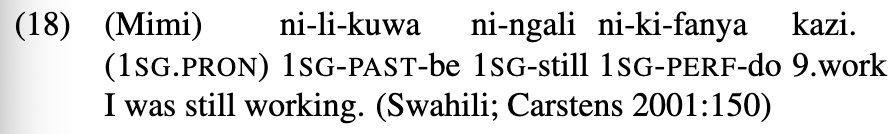
\includegraphics[width=0.57\linewidth]{images/pasted-20260921214721.png}\end{center}

\begin{itemize}
  \item In some languages, a single DP can receive more than one case? (Merchant 2006, Merchant 2011)
\end{itemize}

Two solutions:

\begin{enumerate}
  \item Look for language-specific solutions, and keep the Activity Condition.
  \begin{itemize}
    \item Ferreira 2004 for BP hyperraising with ``defective'' probes
    \item Carstens 2010, Carstens 2011, Carstens and Diercks 2013: Bantu languages lack case features, but have uninterpretable but valued gender features participating in phi-agree - valuedness protects them from deletion, and uninterpretability makes their hosts ``hyperactive'' (able to participate in unlimited number of phi-agreements)
  \end{itemize}
  \item Get rid of the Activity Condition, allowing hyperraising and multiple agreement.
  \begin{itemize}
    \item Analyze English and other similar languages as having factors ruling these things out:
    \begin{itemize}
      \item Nevins 2004 observes that English hyperraising would violate the PIC, but in BP, subjects move slightly higher than they do in English, allowing them to escape the lower phase.
      \item Or Agree in the English hyperraising case violates minimality - English embedded finite CP itself bears phi features (Halpert 2016, Halpert 2019)
    \end{itemize}
  \end{itemize}
\end{enumerate}

Without activity:

\begin{enumerate}
  \item \textbf{Activity condition}: removed
  \item \textbf{Goal flagging, revised}: the goal is assigned a feature indicating agreement with the probe.
\end{enumerate}

\section*{Directionality}

Directionality of movement is well-established as upwards. If Move is just Agree+Merge, then this would make sense if Upwards Agree was banned.

\begin{itemize}
  \item plausibly this follows from cyclicity of structure-building: Rezac 2003, Béjar and Rezac 2009, Preminger 2014, Carstens 2016).
  \begin{itemize}
    \item Agree takes place as soon as the head bearing the probe is Merged -- at this point, only the head and its complement have been constructed, so only material within the complement is available to Agree.
  \end{itemize}
\end{itemize}

Alternatively, Upwards Agree is possible: Zeijlstra 2004, Zejlstra 2008, Zejlstra 2012, Merchant 2006, Merchant 2011, Wurmbrand 2012, Bjorkman and Zeijlstra 2019, Carstens 2016, Baker and Camargo Souza 2020, Arregi and Hanink 2022, etc.

\begin{itemize}
  \item then the ban on lowering would have to come from some constraint on Merge (assuming Move = Merge+Agree)
\end{itemize}

Zeijlstra argues for \textit{only} Upwards Agree based mostly on Negative Concord.

\begin{itemize}
  \item NCIs are a special type of indefinites that Agree with the negation that scopes over them
  \item negation is interpretable with just sentential negation, but not with just NCIs; thus the \textit{interpretable} one is the sentential negation - the goal, the higher thing
  \item this is Upwards Multiple Agree (cuz you can have two probes lower down)
  \item Deal 2022 expands on the typology of negative concord along these lines.
  \item Zeijlstra also treats sequence of tense as agreement, involving only one semantic past tense located in the matrix clause: ``Anjali thought it was snowing''
\end{itemize}

\#me hm actually couldn't you do this the other way around

\begin{itemize}
  \item like, when you're down low, you know that semantically the object is ``nothing'', so you have enough information to output \textit{nessuno}
  \item then, when you're higher up, you know that you need your polarity head to agree with the polarity of the sentence so far - so you agree - the higher thing is still the probe
\end{itemize}
?

\#me also like the sequence of tense thing... can't it just be that the English past tense means ``in the past'' and you don't have to relativize it when you embed? like, you evaluated the embedded \textit{p} on the matrix timeframe

Norwegian and Frisian Parasitic Participle Constructions discussed in Wurmbrand 2012:

\begin{itemize}
  \item the perfect auxiliary ``had'` licenses participial form for not just the main verb but also its complement: ``I had wanted written [=to read] the book''
\end{itemize}

\#me Analyzing Agree as still having to do with uninterpretability maybe explains why negative concord, sequence of tense, and participle licensing contrast with phi-agreement in their directionality: phi-agreement features are interpretable lower (on the DP), and past tense, negatives, etc. are interpretable higher.

But Deal wants to say the opposite: actually you could just analyze these all backwards as downwards Agree.

\section*{Proposal}

Agree seems to have two types of effects:

\begin{enumerate}
  \item features are transferred
  \item movement is triggered
\end{enumerate}

Agree is:

\begin{itemize}
  \item subject to Relativized Minimality
\end{itemize}

Deal argues that Agree is helpful to encode redundancy in communication.

\bigskip

\begin{enumerate}
  \item Probes attend to some features, and not others.
\end{enumerate}
These are the features the probe \textit{interacts} with.

\begin{itemize}
  \item Generally correspond to the ``unvalued'' features in other theories.
  \item Probes stop after seeing some features, and not others.
\end{itemize}
These are the features that \textit{satisfy} the probe.

\begin{itemize}
  \item Probes that never stop agreeing are \textit{insatiable}.
\end{itemize}

\subsection*{Algorithm}

Each syntactic object `H` is specified for interaction features `int(H)` and satisfaction features `sat(H)`.

\begin{enumerate}
  \item The probe does a search through its c-command domain.
  \item For each syntactic object in the search:
  \begin{enumerate}
    \item Determine whether it contains features that should be copied to the probe.
    \item If so:
    \begin{enumerate}
      \item Copy them.
      \item Assign a flag to the target indicating it has interacted with the probe.
      \item If movement is indicated for an interacting feature:
      \begin{enumerate}
        \item Re-merge the target to H's projection.
      \end{enumerate}
    \end{enumerate}
    \item Determine whether the target under consideration should halt, or further probe.
    \item If it should halt:
    \begin{enumerate}
      \item Assign a flag to the target indicating it has satisfied the probe.
      \item If movement has been indicated for a satisfying feature:
      \begin{enumerate}
        \item Re-merge the target to H's position.
      \end{enumerate}
      \item Exit.
    \end{enumerate}
  \end{enumerate}
\end{enumerate}

Questions:

\begin{enumerate}
  \item What is the nature of the search (depth-first or breadth first)? see Branan and Erlewine (To appear)
\end{enumerate}

Example:

\begin{itemize}
  \item H = T
  \item int(H) = all phi-features
  \item sat(H) = all phi-features
\end{itemize}
Thus the first thing H sees with phi-features will copy them all to H. Then, H won't probe anymore, because it'll be satisfied.

\begin{itemize}
  \item When the thing interacts with and satisfies T, it is flagged as T's goal - in English, with NOM.
\end{itemize}
\#me is this from the interaction flag or the satisfaction flag or both?

\begin{itemize}
  \item Given English T's probe specification, this thing must move - meaning either int(T) or sat(T) bears \textasciicircum{}M in English.
\end{itemize}
\#me does int(T) or sat(T) bear \textasciicircum{}M as a whole, or just some elements of them?

More in \textit{dynamic interaction} - Deal 2024.

\subsection*{What this solves}

E.g. for the Churag Darwa case:

\begin{itemize}
  \item the probe is satisfied by [Part]
  \item but interacts with both [Part] and [Spkr]
\end{itemize}

Or for where a probe copies features from multiple targets:

\begin{itemize}
  \item multiple-wh: [int: wh\textasciicircum{}M, sat: -]
  \item agrees with all phi until hits an addressee: [int:phi, sat:addr]
\end{itemize}

NPI agreement is not a problem because there's no tie to semantics.

\#me this is important:

Part of a class of analyses Preminger 2014 describes as Obligatory Operations Models:

\begin{itemize}
  \item It's not that Agree freely applies or not, with the outcome assessed by a series of filters (like uninterpretable features at LF).
  \item Instead, everything is predetermined.
  \item \textit{Because Agree is triggered when the probe is Merged, search proceeds downwards.}
  \item \textit{If Agree `fails', that's fine.}
\end{itemize}

\subsection*{Goal flagging/Node sprouting}

Here, does not require the goal to have anything except the interaction or satisfaction features - no Activity condition, but yes marked afterwards.
